
\chapter{ಸರ್ವೇ ಉಪಕರಣಕ್ಕೆ ದೊರಕಿತು ವಿಶ್ವದ ಅತ್ಯಂತ ಉನ್ನತ ಶಿಖರದ ಎತ್ತರ}

\vskip -12pt

\begin{figure}[!hbtp]
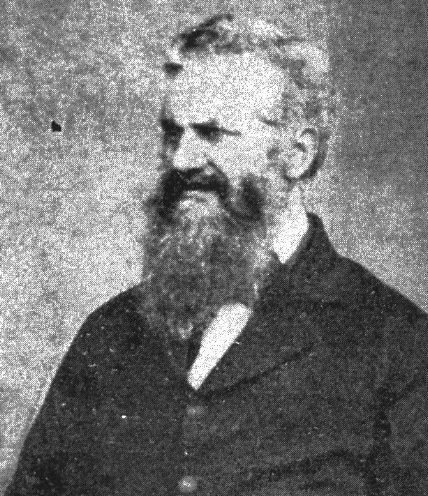
\includegraphics[scale=1.1]{"images/image021.jpg"}
\caption{ಸರ್ ಆಂಡ್ರ್ಯೂ ಸ್ಕಾಟ್‌ವಾಗ್​}\label{chap15-fig1}
\end{figure}

ಆಂಡ್ರ್ಯೂ ವಾಗ್​ರವರು \enginline{1847}ರಲ್ಲಿ, ನಾರ್ಥ್ ಈಸ್ಟರ್ನ್ ಸರಣಿ ಟ್ರಾಂಗ್ಯುಲೇಷನ್​ ಕಾರ್ಯದಲ್ಲಿದ್ದಾಗಲೇ, ಅತಿ ಎತ್ತರದ ಕಾಂಚನಗಂಗಾ ಶಿಖರವನ್ನು ವೀಕ್ಷಣೆ ಮಾಡಿದರು. ಇದು ಪ್ರಪಂಚದ ಮೂರನೇ ಅತಿ ಎತ್ತರದ ಪರ್ವತ. ಇದು \enginline{28126} ಅಡಿ ಎತ್ತರವಿದೆ. ಇದೇ ಸಮಯದಲ್ಲಿ ಅವರು ಡಾರ್ಜಲಿಂಗ್​ನಿಂದ, ಅತ್ಯಂತ ಎತ್ತರವಾಗಿ ಗೋಚರಿಸುತ್ತಿದ್ದ ಇನ್ನೊಂದು ಪರ್ವತ ಶಿಖರಕ್ಕೆ ವೀಕ್ಷಣೆ ಮಾಡಿದರು. ಅದನ್ನು ರೋಮನ್​ ಅಕ್ಷರದಲ್ಲಿ ‘ಗಾಮಾ’ ಎಂದು ಸೂಚಿಸಿದರು. ವೀಕ್ಷಣಾ ಕ್ರಮಾಂಕದಲ್ಲಿ ಈ ಪರ್ವತವನ್ನು \enginline{15}ನೇಯದು ಎಂದೂ ಸಹ ಕರೆಯಲಾಗಿದೆ. ಬೇರಿಂಗನ್ನು ಓದಿ ಆ ‘ಗಾಮಾ’ ಪರ್ವತದ ಸ್ಥಾನವನ್ನು ಆಂಡ್ರ್ಯೂ ವಾಗ್​ರವರು ನಿಗಧಿ ಮಾಡಿದರು. ನಿಂತ ಉಪಕರಣ ತಾಣದಿಂದ ಆ ಪರ್ವತವು ಬಹಳ ದೂರ ಇದ್ದುದರಿಂದ, ಆಗ ಅವರಿಗೆ ಅದರ ಎತ್ತರವನ್ನು ನಿಖರವಾಗಿ ನಿಗಧಿ ಮಾಡಲು ಆಗಲಿಲ್ಲ. ಹಿಮಾಲಯದ ಶಿಖರಗಳು ಬೆಳಗಿನ ಸ್ವಲ್ಪ ಸಮಯದಲ್ಲಷ್ಟೇ ಗೋಚರಿಸುತ್ತಿದ್ದವು. ಅದೂ ನವಂಬರ್​ ಡಿಸೆಂಬರ್​ ತಿಂಗಳಿನಲ್ಲಿ ಮಾತ್ರ. ರಾತ್ರಿಯ ಕತ್ತಲು ಕಳೆಯುವುದನ್ನೇ ಕಾದು, ಬೆಳಿಗ್ಗೆ ಎದ್ದು, ಸ್ಟೇಷನ್​ ಮೇಲೆ ಥಿಯಡೊಲೈಟ್​ ಸ್ಥಾಪಿಸಿ, ಟೆಲಿಸ್ಕೋಪನ್ನು ಅವುಗಳತ್ತ ತಿರುಗಿಸುವಷ್ಟರಲ್ಲಿಯೇ ಅವುಗಳು ಮಂಜು ಮುಸುಕಿ ಮರೆಯಾಗಿಬಿಡುತ್ತಿದ್ದವು. ಅವತ್ತಿನ ದಿನದ ವೀಕ್ಷಣೆ ಅಷ್ಟೇ.

\vskip 4pt

ವಾಗ್​ರವರ ತಂಡದ ಇನ್ನೂ ಅನೇಕರು, ನಾರ್ಥ್ ಈಸ್ಟರ್ನ್ ಸರಣಿಯ ಬೇರೆ ಬೇರೆ ಬೇಸ್‌ಲೈನಿನಿಂದ ಈ ‘ಗಾಮಾ’ ಶಿಖರದ ವೀಕ್ಷಣಾ ಕಾರ್ಯವನ್ನು ಮಾಡಿದರು. \enginline{1850}ರ ಹೊತ್ತಿಗೆ, ಈ ‘ಗಾಮಾ’ ಶಿಖರದ ಮಹಾನ್​ ಔನ್ನತ್ಯವು ವೀಕ್ಷಣೆಯಿಂದ ಗೊತ್ತಾಯಿತು. ವಾಗ್​ರವರು, ಕೊಲ್ಕತ್ತಾದ ತಮ್ಮ ಸಹಾಯಕ, ಚೀಫ್​ ಕಂಪ್ಯೂಟರ್​ರವರನ್ನು ಸಂಪರ್ಕಿಸಿದರು. ನೂರು ಮೈಲು ದೂರದ ಮಂಜಿನ ಶಿಖರಗಳನ್ನು ಪ್ಲಾಟ್​ ಮಾಡಲು ಅವರಿಂದ ಪರಿಷ್ಕೃತ ನಿಯಮಗಳನ್ನು ಕೋರಿದರು. ಆ ಚೀಫ್​ ಕಂಪ್ಯೂಟರ್​ರವರು ಭಾರತದ ರಾಧಾನಾಥ್​ ಸಿಕ್ದರ್​.

\begin{figure}[!hbtp]
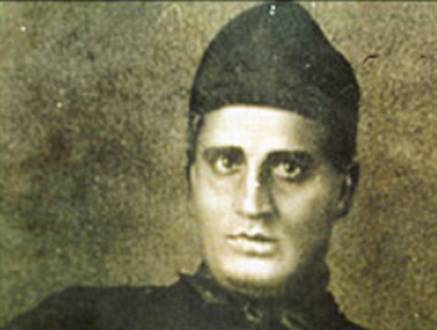
\includegraphics[scale=1.2]{"images/image019.jpg"}
\caption{ರಾಧಾನಾಥ್​ ಸಿಕ್ದರ್​}\label{chap15-fig2}
\end{figure}

ರಾಧಾನಾಥ್​ ಸಿಕ್ದರ್​ರವರು ಬೆಂಗಾಳಿ ಮಹಾ ಪ್ರತಿಭೆ. ಗಣಿತ ಮಾಂತ್ರಿಕ. ಇವರ ಅದ್ಭುತ ಗಣಿತ ಶಕ್ತಿ ಎವರೆಸ್ಟ್​ರವರನ್ನು ಸಹ ಪ್ರಭಾವಿಸಿತ್ತು. ಕ್ಷೇತ್ರ ಕಾರ್ಯದ ನೂರಾರು ವೀಕ್ಷಣೆಗಳನ್ನು ಪಡೆದು, \enginline{1852}ರಲ್ಲಿ ರಾಧಾನಾಥ್​ ಸಿಕ್ದರ್​ರವರು ಹಿಮಾಲಯ ಎತ್ತರವನ್ನು ತಮ್ಮ ಅಪ್ರತಿಮ ಗಣಿತ ಶಕ್ತಿ ಉಪಯೋಗಿಸಿ ಲೆಕ್ಕಾಚಾರ ಮಾಡಿದರು. ವಿಶ್ವದ ಅತ್ಯಂತ ಉನ್ನತ ಶಿಖರದ ಮೊದಲ ಖಚಿತ ಲೆಕ್ಕಾಚಾರ ಅವರದೇ. ಸಡಗರ ಸಂಭ್ರಮದಲ್ಲಿ ವಾಗ್​ರವರ ಕಛೇರಿಗೆ ನುಗ್ಗಿ ವಿಶ್ವದಾಖಲೆಯ ಪರ್ವತದ ಎತ್ತರವನ್ನು ಘೋಷಿಸಿದರು. ಆದರೆ ವಾಗ್​ರವರು ಆತುರದಲ್ಲಿ ಇರಲಿಲ್ಲ.

 ಸರ್ವೇಗೂ ಸಂಹಿತೆ ಎಂಬುದು ಇದೆ. ಸರ್ವೇ ಅಂದರೆ ಅದು ಸರಳವಾದುದು ಅಲ್ಲ. ಅದು ಸಂಕೀರ್ಣ ಪ್ರಕ್ರಿಯೆ. ಪರಿಶೀಲನೆ ಮಾಡದೆ, ತಾಳೆ ನೋಡದೆ ಯಾವ ಹೊಸ ಶೋಧನೆಯನ್ನೂ ಪ್ರಕಟಿಸುವಂತಿರಲಿಲ್ಲ. ನಕ್ಷೆಯಲ್ಲಿನ ಪ್ರತಿ ಗೆರೆ, ರೇಖೆಯ ಹಿಂದೆ ಕರಾರುವಕ್ಕಾದ ಪರಿಶೀಲನೆ, ಅನುಭವ ಇರುತ್ತದೆ. ಎಲ್ಲರೂ ಒಪ್ಪಿ ಸ್ವೀಕರಿಸುವ ಸಂಪೂರ್ಣ ಗಣಿತ ತರ್ಕ, ಲೆಕ್ಕಾಚಾರ ಇರುತ್ತದೆ. ಟ್ರಿಗನಮಿಟ್ರಿಕಲ್​ ಸರ್ವೇಯೊಂದೇ ವಿಶ್ವದ ಅತ್ಯಂತ ಉನ್ನತವಾದ ಈ ಶಿಖರದ ಖಚಿತ ಲೆಕ್ಕಾಚಾರಕ್ಕೆ ಸಮರ್ಪಕವಾದ ಗಣಿತ ವಿವರಣೆಯನ್ನು ನೀಡಲು ಗಟ್ಟಿಯಾದ ಆಧಾರವನ್ನು ಒದಗಿಸಿತ್ತು.

ಮುಂದಿನ ನಾಲ್ಕು ವರ್ಷಗಳು ವಕ್ರೀಭವನ ಗುಣಾಂಕ, ಸರಾಸರಿ ಸಮುದ್ರಮಟ್ಟದ ಡೇಟಮ್‌ನ ನಿಗಧಿ, ಲೆಕ್ಕಾಚಾರದ ಪರಿಶೀಲನೆ, ಮರು ಪರಿಶೀಲನೆ, ಹಿಂದಿನ ವೀಕ್ಷಣೆಗಳ ಪರಿಶೀಲನೆ ಇವುಗಳಲ್ಲಿ ಕಳೆಯುತ್ತದೆ. ಮಾರ್ಚ್ \enginline{1856}ರಲ್ಲಿ ಆಂಡ್ರ್ಯೂ ವಾಗ್​ರವರು, ಅಂತಿಮವಾಗಿ ಅವರ ಸಹಾಯಕ, ಡೆಪ್ಯೂಟಿ ಸರ್ವೇಯರ್​ ಜನರಲ್​, ಕ್ಯಾಪ್ಟನ್​ ತುಯ್​ಲಿಯರ್​\break ರವರಿಗೆ ಬರೆದು, ಗಾಮ ಸಂಕೇತಾಕ್ಷರ ಹೊಂದಿದ ಪರ್ವತದ ವಿಶ್ವದಾಖಲೆಯ ಎತ್ತರವನ್ನು ಪ್ರಕಟಿಸುವಂತೆ ತಿಳಿಸಿದರು.

\begin{figure}[!htbp]
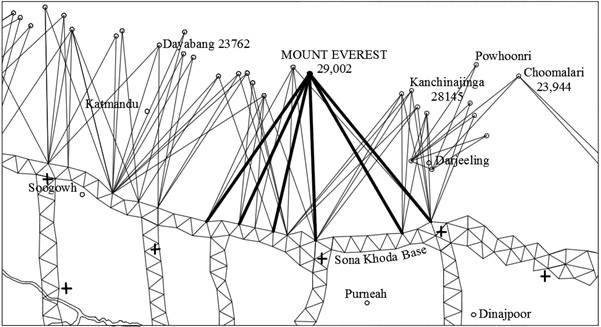
\includegraphics{"images/image020.jpg"}
\caption{ನಾರ್ಥ್ ಈಸ್ಟರ್ನ್ ಸರಣಿಯ ವಿವಿಧ ಬೇಸ್‌ಲೈನಿನಿಂದ ಮೌಂಟ್​ ಎವರೆಸ್ಟ್​ಗೆ ವೀಕ್ಷಣೆ}\label{art15-fig2}
\end{figure}

\newpage

ವಿಶ್ವದ ಅತ್ಯಂತ ಎತ್ತರದ ಆ ಶಿಖರದ ಬಗ್ಗೆ ಆಂಡ್ರ್ಯೂ ವಾಗ್​ರವರು ಬರೆದು ದಾಖಲಿಸಿದ ನಿರ್ಣಯಗಳನ್ನು ನೊಡಿ. “ಈ ಪರ್ವತವು ಭಾರತದಲ್ಲಿ ಅಳತೆ ಮಾಡಲಾದ ಉಳೆದೆಲ್ಲ ಪರ್ವತಗಳಿಗಿಂತ ಎತ್ತರವಾದ ಪರ್ವತ. ಅಷ್ಟೇ ಅಲ್ಲ, ವಿಶ್ವದಲ್ಲಿಯೇ ಎತ್ತರವಾದ ಪರ್ವತವಾಗಿದೆ. ಪ್ರತಿಯೊಂದು ಪ್ರಮುಖ ಭೌಗೋಳಿಕ ವಿವರವನ್ನು ಅದರ ಸ್ಥಳೀಯ ಹೆಸರಿನಿಂದಲೇ ಗುರುತಿಸಬೇಕೆಂದು ಗೌರವಾನ್ವಿತ ಕರ್ನಲ್​ ಜಾರ್ಜ್ ಎವರೆಸ್ಟ್​ರವರ ಸ್ಪಷ್ಟ ಅಭಿಪ್ರಾಯ. ಆದರೆ ವಿಶ್ವದ ಅತಿ ಎತ್ತರದ ಈ ಪರ್ವತಕ್ಕೆ ನಮಗೆ ಸ್ಥಳೀಯ ಹೆಸರು ಇನ್ನೂ ಸಿಕ್ಕಿಲ್ಲ. ನೇಪಾಳ ದೇಶಕ್ಕೆ ಪ್ರವೇಶಿಸುವ ಅನುಮತಿ ಸಿಕ್ಕ ನಂತರವಷ್ಟೇ, ಆ ಹಿಮಪ್ರದೇಶಕ್ಕೆ ಇರಬಹುದಾದ ಸ್ಥಳೀಯ ಹೆಸರನ್ನು ಖಚಿತಪಡಿಸಿಕೊಳ್ಳಲು ಸಾಧ್ಯ. ವಿಶ್ವದ ಅತಿ ಎತ್ತರದ ಈ ಶಿಖರಕ್ಕೆ ಶಾಶ್ವತವಾದ ಒಂದು ಹೆಸರನ್ನು ಸೂಚಿಸುವುದು ನನ್ನ ಕರ್ತವ್ಯ ಮತ್ತು ಸುಯೋಗವಾಗಿದೆ. ಈ ನಮ್ಮ ಗ್ರೇಟ್​ ಟ್ರಿಗನಮಿಟ್ರಿಕಲ್​ ಸರ್ವೇಯ ಪ್ರಗತಿಗಾಗಿ ಅಪಾರವಾಗಿ ದುಡಿದ, ಮಹನೀಯರಾದ ಕರ್ನಲ್​ ಜಾರ್ಜ್ ಎವರೆಸ್ಟ್​ರವರ ಮಹಾ ಕೊಡುಗೆಯ ಮೇಲಿನ ಗೌರವದ ಸಂಕೇತವಾಗಿ ಮತ್ತು ಸರ್ವೇ ಆಫ್​ ಇಂಡಿಯಾ ಮಹಾನ್​ ವಿಜ್ಞಾನ ಸಂಸ್ಥೆಯ ಎಲ್ಲರ ಆಶಯದಂತೆ, ಈ ಸಂಸ್ಥೆಯ ಮುಖ್ಯಸ್ಥನಾಗಿ, ಈ ಮಹಾನ್​ ಶಿಖರಕ್ಕೆ ‘ ಮೌಂಟ್​ ಎವರೆಸ್ಟ್​’ ಎಂದು ಹೆಸರಿಸಲು ನಿರ್ಣಯಿಸಿದ್ದೇನೆ. ಈ ಶಿಖರದ ಭೌಗೋಳಿಕ ಸ್ಥಾನದ ಕೋಆರ್ಡಿನೇಟ್​, ಸಮಭಾಜಕದಿಂದ \enginline{270 59}’ \enginline{16.7}” ಉತ್ತರ, ಗ್ರೀನ್​ವಿಚ್​ನ ಪ್ರಧಾನ ರೇಖಾಂಶದಿಂದ \enginline{860 58}’ \enginline{5.9}” ಪೂರ್ವ ಮತ್ತು ಸರಾಸರಿ ಸಮುದ್ರಮಟ್ಟದಿಂದ \enginline{29002} ಅಡಿ ಎತ್ತರ ಆಗಿರುತ್ತದೆ”.

ಕೊಲ್ಕೊತ್ತಾದಲ್ಲಿನ ಏಸಿಯಾಟಿಕ್​ ಸೊಸೈಟಿಯ ಸದಸ್ಯರಿಗೆ ಕ್ಯಾಪ್ಟನ್​ ತುಯ್​ಲಿಯರ್​\-ರವರು ಈ ನಿರ್ಣಯವನ್ನು ರವಾನಿಸುತ್ತಾರೆ. ಏಸಿಯಾಟಿಕ್​ ಸೊಸೈಟಿಯು, ಹೆಸರನ್ನು ಹೊರತುಪಡಿಸಿ, ಆಂಡ್ರ್ಯೂ ವಾಗ್​ರವರ ಉಳಿದೆಲ್ಲಾ ಅಂಶಗಳನ್ನು ಒಪ್ಪಿಕೊಳ್ಳುತ್ತದೆ. ಲಂಡನ್ನಿನ ಸೆಕ್ರಟರಿ ಆಫ್​ ಸ್ಟೇಟ್​ ಫಾರ್​ ಇಂಡಿಯಾ ಮತ್ತು ರಾಯಲ್​ ಜೀಯಾಗ್ರಫಿಕಲ್​ ಸೊಸೈಟಿಗಳು ಈ ಹೆಸರನ್ನು ಸಮ್ಮತಿಸಿ, ಒಪ್ಪಿಗೆ ನೀಡುತ್ತವೆ. ಇಡೀ ವಿಶ್ವದ ಅತೀ ಎತ್ತರದ ‘ಗಾಮಾ’ ಶಿಖರಕ್ಕೆ, ಈ ರೀತಿಯಾಗಿ ‘ ಮೌಂಟ್​ ಎವರೆಸ್ಟ್​’ ಎಂದು \enginline{1856} ರಲ್ಲಿ ಹೊಸದಾಗಿ ನಾಮಕರಣ ವಾಗುತ್ತದೆ.

‘ಗಾಮಾ’ ಶಿಖರಕ್ಕೆ ಎವರೆಸ್ಟ್​ರವರ ಹೆಸರು ಇರಿಸಿದ ಕ್ರಮದ ಸರಿ ತಪ್ಪುಗಳ ಬಗ್ಗೆ ಚರ್ಚೆ ನಡೆಯಿತು. ನೇಪಾಳದಲ್ಲಿ `ಮೌಂಟ್​ ಎವರೆಸ್ಟ್​’ ಪರ್ವತವನ್ನು ‘ದೇವಧಾಂಗ’ ಎಂದು ಕರೆಯುತ್ತಾರೆ, ಆದ್ದರಿಂದ ಆ ಹೆಸರೇ ಸೂಕ್ತವೆಂದು ಕೆಲವರ ಅಭಿಪ್ರಾಯ. ಆದರೆ, ‘ದೇವಧಾಂಗ’ ವೆಂದರೆ ಅದು ಒಟ್ಟು ಶಿಖರಗಳ ಸಮುಚ್ಚಯಕ್ಕೆ ಇರುವ ಹೆಸರು, ಒಂದು ಶಿಖರಕ್ಕಲ್ಲ ಎಂಬ ಕಾರಣದಿಂದ ಈ ಹೆಸರು ಸ್ವೀಕಾರವಾಗುವುದಿಲ್ಲ.

ಟಿಬೆಟಿಯನ್​ನಲ್ಲಿ ಈ ಪರ್ವತಕ್ಕೆ ‘ಚಾ–ಮೊ–ಲುಂಗ್​–ಮಾ’ ಎಂಬ ಹೆಸರು ಇದೆ. ಆದರೆ ಇದೂ ಸಹ ಪರ್ವತಗಳ ಇಡೀ ಪ್ರದೇಶಕ್ಕೆ ಸೂಚಿತವಾದ ಹೆಸರು. ಈ ಕಾರಣಕ್ಕೆ ಈ ಹೆಸರೂ ಒಪ್ಪಿಗೆ ಪಡೆಯುವುದಿಲ್ಲ. ಟಿಬೆಟ್ಟಿಯನ್​ನಲ್ಲಿ ಈ ಪರ್ವತಕ್ಕೆ ಇನ್ನೂ ಒಂದು ಉದ್ದವಾದ ಹೆಸರಿದೆ. ‘ಮಿ–ಥಿಕ್​–ದ್ಗು–ಬ್ಯಾ–ಫರ್​–ಲಾಂಗ್​–ನ್ಗಾ’ ಎಂದು. ಭಾಷಂತರಿಸಿದರೆ ಇದರ ತಾತ್ಪರ್ಯವು ‘ಹತ್ತಿರದಿಂದ ನೀವು ಈ ಶಿಖರವನ್ನು ನೋಡಲಾರಿರಿ, ಆದರೂ ನವ ದಿಕ್ಕಿನಲ್ಲೂ ಇದು ಗೋಚರ. ಇದರೆತ್ತರಕ್ಕೆ ಹಾರುವ ಹಕ್ಕಿಗೆ ಮತ್ತೇನೂ ಕಾಣದು’. ಮ್ಯಾಪಿಂಗ್​ಗೆ ಇಷ್ಟು ಉದ್ದವಾದ ಪದಪುಂಜ ಸೂಕ್ತವಲ್ಲವೆಂದು ಈ ಹೆಸರೂ ಸ್ವೀಕಾರ ಆಗುವುದಿಲ್ಲ. ‘ಮೌಂಟ್​​ ಎವರೆಸ್ಟ್​’ ಹೆಸರು ಮಾತ್ರ ಬದಲಾಗದೇ ಉಳಿಯಿತು. ಈ ರೀತಿಯಾಗಿ, \enginline{1856} ರಲ್ಲಿ ಹೊಸದಾಗಿ ವಿಶ್ವ ಶ್ರೇಷ್ಠ ಸರ್ವೇಯರ್​ ಒಬ್ಬರ ಹೆಸರಿನಲ್ಲಿ ನಾಮಕರಣವಾದ, `ಮೌಂಟ್​ ಎವರೆಸ್ಟ್​’ ಎಂಬ ಪದವೇ ಇಂದು ವಿಶ್ವಮಾನ್ಯವಾಗಿದೆ. ಇಡೀ ವಿಶ್ವದ ಅತಿ ಎತ್ತರದ ಶಿಖರಕ್ಕೆ ತನ್ನ ಹೆಸರನ್ನು ಇಟ್ಟ ಬಗ್ಗೆ ಸ್ವತಃ ಜಾರ್ಜ್ ಎವರೆಸ್ಟ್​ರವರು ಯಾವೊಂದು ಪ್ರತಿಕ್ರಿಯೆ ನೀಡಿದ ಬಗ್ಗೆ ದಾಖಲಾಗಿಲ್ಲ. ಈ ಬಗ್ಗೆ ಅವರ ಮೌನವೂ ಸಹ ಅನೇಕರಿಗೆ ಕುತೂಹಲದ ವಿಷಯವಾಗಿದೆ.

